% hw2.tex

% !TEX program = xelatex
%%%%%%%%%%%%%%%%%%%%
% see http://mirrors.concertpass.com/tex-archive/macros/latex/contrib/tufte-latex/sample-handout.pdf
% for how to use tufte-handout
\documentclass[a4paper, justified]{tufte-handout}
\usepackage{tikz}
\usetikzlibrary{arrows,automata}
\usepackage{amsmath}


% hw-preamble.tex

% geometry for A4 paper
% See https://tex.stackexchange.com/a/119912/23098
\geometry{
  left=20.0mm,
  top=20.0mm,
  bottom=20.0mm,
  textwidth=130mm, % main text block
  marginparsep=5.0mm, % gutter between main text block and margin notes
  marginparwidth=50.0mm % width of margin notes
}

% for colors
\usepackage{xcolor} % usage: \color{red}{text}
% predefined colors
\newcommand{\red}[1]{\textcolor{red}{#1}} % usage: \red{text}
\newcommand{\blue}[1]{\textcolor{blue}{#1}}
\newcommand{\teal}[1]{\textcolor{teal}{#1}}

\usepackage{todonotes}

% heading
\usepackage{sectsty}
\setcounter{secnumdepth}{2}
\allsectionsfont{\centering\huge\rmfamily}

% for Chinese
\usepackage{xeCJK}
\usepackage{zhnumber}
\setCJKmainfont[BoldFont=FandolSong-Bold.otf]{FandolSong-Regular.otf}

% for fonts
\usepackage{fontspec}
\newcommand{\song}{\CJKfamily{song}}
\newcommand{\kai}{\CJKfamily{kai}}

% To fix the ``MakeTextLowerCase'' bug:
% See https://github.com/Tufte-LaTeX/tufte-latex/issues/64#issuecomment-78572017
% Set up the spacing using fontspec features
\renewcommand\allcapsspacing[1]{{\addfontfeature{LetterSpace=15}#1}}
\renewcommand\smallcapsspacing[1]{{\addfontfeature{LetterSpace=10}#1}}

% for url
\usepackage{hyperref}
\hypersetup{colorlinks = true,
  linkcolor = teal,
  urlcolor  = teal,
  citecolor = blue,
  anchorcolor = blue}

\newcommand{\me}[4]{
    \author{
      {\bfseries 姓名:}\underline{#1}\hspace{2em}
      {\bfseries 学号:}\underline{#2}\hspace{2em}\\[10pt]
      {\bfseries 评分:}\underline{#3\hspace{3em}}\hspace{2em}
      {\bfseries 评阅:}\underline{#4\hspace{3em}}
  }
}

% Please ALWAYS Keep This.
\newcommand{\noplagiarism}{
  \begin{center}
    \fbox{\begin{tabular}{@{}c@{}}
      请独立完成作业,不得抄袭。\\
      若得到他人帮助, 请致谢。\\
      若参考了其它资料,请给出引用。\\
      鼓励讨论,但需独立书写解题过程。
    \end{tabular}}
  \end{center}
}

% \newcommand{\goal}[1]{
%   \begin{center}{\fcolorbox{blue}{yellow!60}{\parbox{0.50\textwidth}{\large
%     \begin{itemize}
%       \item 体会``思维的乐趣''
%       \item 初步了解递归与数学归纳法
%       \item 初步接触算法概念与问题下界概念
%     \end{itemize}}}}
%   \end{center}
% }

% Each hw consists of four parts:
\newcommand{\beginrequired}{\hspace{5em}\section{作业 (必做部分)}}
\newcommand{\beginoptional}{\section{作业 (选做部分)}}
\newcommand{\beginot}{\section{Open Topics}}
\newcommand{\begincorrection}{\section{订正}}
\newcommand{\beginfb}{\section{反馈}}

% for math
\usepackage{amsmath, mathtools, amsfonts, amssymb}
\newcommand{\set}[1]{\{#1\}}

% define theorem-like environments
\usepackage[amsmath, thmmarks]{ntheorem}

\theoremstyle{break}
\theorempreskip{2.0\topsep}
\theorembodyfont{\song}
\theoremseparator{}
\newtheorem{problem}{题目}[subsection]
\renewcommand{\theproblem}{\arabic{problem}}
\newtheorem{ot}{Open Topics}

\theorempreskip{3.0\topsep}
\theoremheaderfont{\kai\bfseries}
\theoremseparator{:}
\theorempostwork{\bigskip\hrule}
\newtheorem*{solution}{解答}
\theorempostwork{\bigskip\hrule}
\newtheorem*{revision}{订正}

\theoremstyle{plain}
\newtheorem*{cause}{错因分析}
\newtheorem*{remark}{注}

\theoremstyle{break}
\theorempostwork{\bigskip\hrule}
\theoremsymbol{\ensuremath{\Box}}
\newtheorem*{proof}{证明}

% \newcommand{\ot}{\blue{\bf [OT]}}

% for figs
\renewcommand\figurename{图}
\renewcommand\tablename{表}

% for fig without caption: #1: width/size; #2: fig file
\newcommand{\fig}[2]{
  \begin{figure}[htbp]
    \centering
    \includegraphics[#1]{#2}
  \end{figure}
}
% for fig with caption: #1: width/size; #2: fig file; #3: caption
\newcommand{\figcap}[3]{
  \begin{figure}[htbp]
    \centering
    \includegraphics[#1]{#2}
    \caption{#3}
  \end{figure}
}
% for fig with both caption and label: #1: width/size; #2: fig file; #3: caption; #4: label
\newcommand{\figcaplbl}[4]{
  \begin{figure}[htbp]
    \centering
    \includegraphics[#1]{#2}
    \caption{#3}
    \label{#4}
  \end{figure}
}
% for margin fig without caption: #1: width/size; #2: fig file
\newcommand{\mfig}[2]{
  \begin{marginfigure}
    \centering
    \includegraphics[#1]{#2}
  \end{marginfigure}
}
% for margin fig with caption: #1: width/size; #2: fig file; #3: caption
\newcommand{\mfigcap}[3]{
  \begin{marginfigure}
    \centering
    \includegraphics[#1]{#2}
    \caption{#3}
  \end{marginfigure}
}

\usepackage{fancyvrb}

% for algorithms
\usepackage[]{algorithm}
\usepackage[]{algpseudocode} % noend
% See [Adjust the indentation whithin the algorithmicx-package when a line is broken](https://tex.stackexchange.com/a/68540/23098)
\newcommand{\algparbox}[1]{\parbox[t]{\dimexpr\linewidth-\algorithmicindent}{#1\strut}}
\newcommand{\hStatex}[0]{\vspace{5pt}}
\makeatletter
\newlength{\trianglerightwidth}
\settowidth{\trianglerightwidth}{$\triangleright$~}
\algnewcommand{\LineComment}[1]{\Statex \hskip\ALG@thistlm \(\triangleright\) #1}
\algnewcommand{\LineCommentCont}[1]{\Statex \hskip\ALG@thistlm%
  \parbox[t]{\dimexpr\linewidth-\ALG@thistlm}{\hangindent=\trianglerightwidth \hangafter=1 \strut$\triangleright$ #1\strut}}
\makeatother

% for footnote/marginnote
% see https://tex.stackexchange.com/a/133265/23098
\usepackage{tikz}
\newcommand{\circled}[1]{%
  \tikz[baseline=(char.base)]
  \node [draw, circle, inner sep = 0.5pt, font = \tiny, minimum size = 8pt] (char) {#1};
}
\renewcommand\thefootnote{\protect\circled{\arabic{footnote}}}

\newcommand{\score}[1]{{\bf [#1 分]}}

\newcommand{\rel}[1]{\xrightarrow{#1}}
\newcommand{\dstar}{\xRightarrow[]{\ast}}
\newcommand{\dplus}{\xRightarrow[]{+}}
\newcommand{\lm}{\xRightarrow[\text{lm}]{}}
\renewcommand{\rm}{\xRightarrow[\text{rm}]{}}
\newcommand{\dpluslm}{\xRightarrow[\text{lm}]{+}}
\newcommand{\dstarlm}{\xRightarrow[\text{lm}]{\ast}}
\newcommand{\dplusrm}{\xRightarrow[\text{rm}]{+}}
\newcommand{\dstarrm}{\xRightarrow[\text{rm}]{\ast}}

\newcommand{\sep}{\;\big\lvert\;}

\newcommand{\first}{\textsc{First}}
\newcommand{\follow}{\textsc{Follow}}

% see https://tex.stackexchange.com/a/109906/23098
\usepackage{empheq}
\newcommand*\widefbox[1]{\fbox{\hspace{2em}#1\hspace{2em}}} % feel free to modify this file if you understand LaTeX well
%%%%%%%%%%%%%%%%%%%%
\title{编译原理作业 (2)}
\me{魏恒峰}{hfwei@nju.edu.cn}{}{}
\date{2021年11月12日}
%%%%%%%%%%%%%%%%%%%%
\begin{document}
\maketitle
%%%%%%%%%%%%%%%%%%%%
\noplagiarism % PLEASE DON'T DELETE THIS LINE!
%%%%%%%%%%%%%%%%%%%%
\begin{abstract}
  % \mfigcap{width = 0.85\textwidth}{figs/George-Boole}{George Boole}
  % \begin{center}{\fcolorbox{blue}{yellow!60}{\parbox{0.65\textwidth}{\large
  %   \begin{itemize}
  %     \item
  %   \end{itemize}}}}
  % \end{center}
\end{abstract}
%%%%%%%%%%%%%%%%%%%%
\beginrequired
%%%%%%%%%%%%%%%

%%%%%%%%%%%%%%%
\begin{problem}[子集构造法的最坏情况 \score{10 = 4 + 6}]
 请给出识别如下语言的 NFA (以 $n = 3$ 为例), 并使用子集构造法得到等价的 DFA:
    \sidenote{
      如何用 \LaTeX{} 画自动机?
      \begin{itemize}
        \item \href{https://www3.nd.edu/~kogge/courses/cse30151-fa17/Public/other/tikz\_tutorial.pdf}{使用{\texttt{tikz automata}} library}
        \item \href{https://hayesall.com/blog/latex-automata/}{另一个关于\texttt{tikz automata}的教程}
        \item 在\href{https://notendur.hi.is/aee11/automataLatexGen/}{网站\texttt{automataLatexGen}生成\LaTeX{}代码}
        \item 使用教学立方中上传的 \href{https://www.jflap.org/}{\texttt{jflap}} 工具
      \end{itemize}}
  ``长度为 $m \ge n$ 个字符的 $a, b$ 串, 且倒数第 $n$ 个字符是 $a$''。

  \vspace{5pt}
  \noindent 请给出关键的中间步骤以及 DFA 状态与 NFA 状态之间的对应关系。
  不必给出所有的细节, 类似的步骤可以``跳步''。

  \begin{solution}
  $L_3=(a|b)^*a(a|b)(a|b)$\\
  NFA如下:\\
  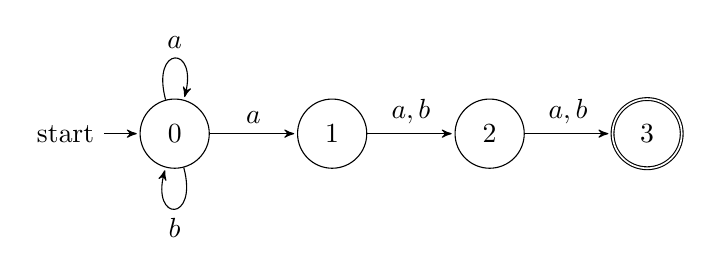
\begin{tikzpicture}[->,>=stealth',shorten >=1pt,auto,node distance=2cm,
        scale = 1,transform shape]

    \node[state,initial] (0) {$0$};
    \node[state] (1) [right of=0] {$1$};
    \node[state] (2) [ right of=1] {$2$};
    \node[state,accepting] (3) [right of=2] {$3$};

    \path (0) edge              node {$a$} (1)
        (0)  edge[loop above]           node {$a$} (0)
        (0)  edge[loop below]           node {$b$} (0)
        (1) edge              node {$a,b$} (2)
        (2) edge              node {$a,b$} (3);

    \end{tikzpicture}\\
    
     \noindent
    $\epsilon-closure(0)=\{0\}$\\
    $\epsilon-closure(move(A,a))=\{0,1\}$\\
    $\epsilon-closure(move(B,a))=\{0,1,2\}$\\
    $\epsilon-closure(move(B,b))=\{0,2\}$\\
    $\epsilon-closure(move(C,a))=\{0,1,2,3\}$\\
    $\epsilon-closure(move(C,b))=\{0,2,3\}$\\
    $\epsilon-closure(move(D,a))=\{0,1,3\}$\\
    $\epsilon-closure(move(D,b))=\{0,3\}$\\
    
    \begin{table}[ht]
    \begin{tabular}{|l|l|l|l|l|}
    \hline
    \textbf{NFA状态} & \textbf{DFA状态} & \textbf{a} & \textbf{b}  \\ \hline
    {0}              & A                & B          & A           \\ \hline
    {0,1}            & B                & C          & D           \\ \hline
    {0,1,2}          & C                & E          & F           \\ \hline
    {0,2}            & D                & G          & H           \\ \hline
    {0,1,2,3}        & E                & E          & F           \\ \hline
    {0,2,3}          & F                & G          & H           \\ \hline
    {0,1,3}          & G                & C          & D           \\ \hline
    {0,3}            & H                & B          & A           \\ \hline
    \end{tabular}
    \end{table}
    
    DFA如下:\\
    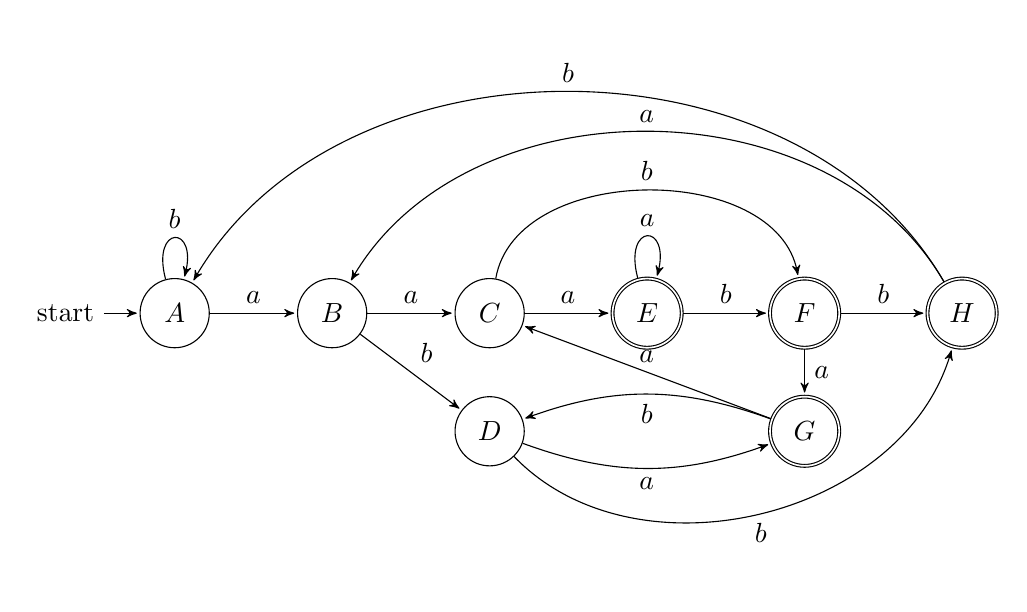
\begin{tikzpicture}[->,>=stealth',shorten >=1pt,auto,node distance=2cm,
        scale = 1,transform shape]
    \node[state,initial] (A) {$A$};
    \node[state] (B) [right of=A] {$B$};
    \node[state] (C) [right of=B] {$C$};
    \node[state] (D) [below of=C,yshift=0.5cm] {$D$};
   
    
    \node[state,accepting] (E) [right of=C] {$E$};
    \node[state,accepting] (F) [right of=E] {$F$};
     \node[state,accepting] (G) [below of=F,yshift=0.5cm] {$G$};
    \node[state,accepting] (H) [right of=F] {$H$};

    \path (A) edge              node {$a$} (B)
        (A)  edge[loop above]           node {$b$} (A)
        (B) edge              node {$a$} (C)
        (B) edge              node {$b$} (D)
        (C) edge              node {$a$} (E)
        (C) edge[above,bend left=80]              node {$b$} (F)
        (D) edge[below,bend right=20]              node {$a$} (G)
        (D) edge[below,bend right=60]              node {$b$} (H)
        (E) edge[loop above]             node {$a$} (G)
        (E) edge              node {$b$} (F)
        (F) edge              node[right] {$a$} (G)
        (F) edge              node {$b$} (H)
        (G) edge              node[above] {$a$} (C)
        (G) edge[above,bend right=20]             node[below] {$b$} (D)
        (H) edge[above,bend right=60]              node {$a$} (B)
        (H) edge[above,bend right=60]              node {$b$} (A);

    \end{tikzpicture}\\
  \end{solution}
\end{problem}
%%%%%%%%%%%%%%%

%%%%%%%%%%%%%%%
\begin{problem}[正则表达式与自动机 \score{10 = 2 + 2 + 2 + 2 + 2}]
  考虑正则表达式 $r = 0^{\ast}10^{\ast}$ (字母表 $\Sigma = \set{0, 1}$)。
  \sidenote{
    如何用 \LaTeX{} 写(复杂的)正则表达式?
    \begin{itemize}
      \item \href{https://tex.stackexchange.com/a/162122/23098}{How to escape properly and output regex in latex?@tex.stackexchange}
    \end{itemize}
  }
  \begin{enumerate}[(1)]
    \item 使用 Thompson 构造法构造等价的 NFA;
    \item 使用子集构造法构造等价的 DFA;
    \item 将上一步构造的 DFA 最小化;
    \item 将上一步得到的最小 DFA 转化为等价的正则表达式, 记为 $r'$ (下周二会介绍该算法)。
    \item $r'$ 与 $r$ 相同吗? 若不同, 请将 $r'$ 转化为 $r$。
  \end{enumerate}
  以上各小题, 请给出关键的中间步骤。

  \noindent (不必给出所有的细节, 类似的步骤可以``跳步''; 尽量将解答部分控制在两页以内。)

\end{problem}

\begin{solution}
(1)\\
\textcircled{1}\quad{$0^*$}\\
% \begin{figure}[h]
    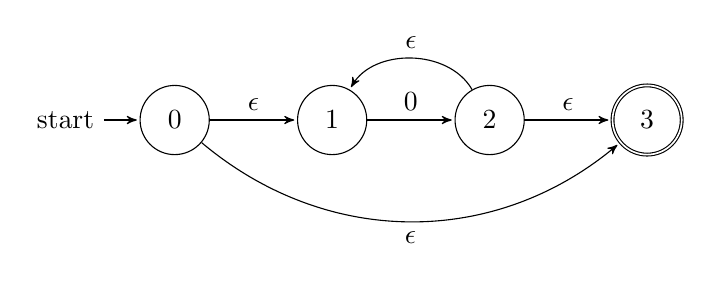
\begin{tikzpicture}[->,>=stealth',shorten >=1pt,auto,node distance=2cm,
        scale = 1,transform shape]

    \node[state,initial] (0) {$0$};
    \node[state] (1) [right of=0]  {$1$};
    \node[state] (2) [right of=1]  {$2$};
    \node[state,accepting] (3) [right of=2] {$3$};

    \path (0) edge              node {$\epsilon$} (1);
    \path (0) edge[below,bend right=40]  node {$\epsilon$} (3);
    \path (1) edge              node {$0$} (2);
    \path (2) edge[above,bend right=60]              node {$\epsilon$} (1);
    \path (2) edge              node {$\epsilon$} (3);

    \end{tikzpicture}
    % \end{figure}
    
  
\textcircled{2}\quad{$0^*10^*$}\\
    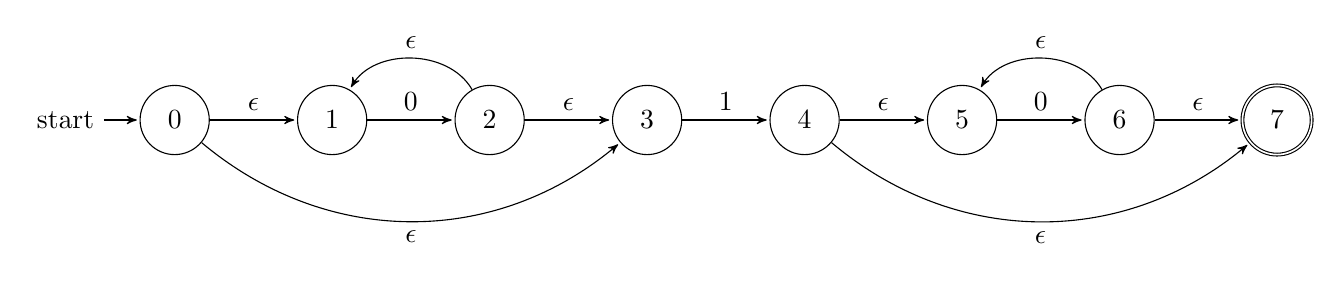
\begin{tikzpicture}[->,>=stealth',shorten >=1pt,auto,node distance=2cm,
        scale = 1,transform shape]

    \node[state,initial] (0) {$0$};
    \node[state] (1) [right of=0]  {$1$};
    \node[state] (2) [right of=1]  {$2$};
    \node[state] (3) [right of=2]  {$3$};
    \node[state] (4) [right of=3]  {$4$};
    \node[state] (5) [right of=4]  {$5$};
    \node[state] (6) [right of=5]  {$6$};
    \node[state,accepting] (7) [right of=6] {$7$};

    \path (0) edge              node {$\epsilon$} (1);
    \path (0) edge[below,bend right=40]  node {$\epsilon$} (3);
    \path (1) edge              node {$0$} (2);
    \path (2) edge[above,bend right=60]              node {$\epsilon$} (1);
    \path (2) edge              node {$\epsilon$} (3);
    \path (3) edge              node {$1$} (4);
    \path (4) edge              node {$\epsilon$} (5);
    \path (4) edge[below,bend right=40]  node {$\epsilon$} (7);
    \path (5) edge              node {$0$} (6);
    \path (6) edge[above,bend right=60]              node {$\epsilon$} (5);
    \path (6) edge              node {$\epsilon$} (7);

    \end{tikzpicture}
\noindent(2)\\
    $\epsilon-closure(0)=\{0,1,3\}$\\
    $\epsilon-closure(move(A,0))=\{1,2,3\}$\\
    $\epsilon-closure(move(A,1))=\{4,5,7\}$\\
    $\epsilon-closure(move(C,0))=\{5,6,7\}$\\
    
    \begin{table}[ht]
    \begin{tabular}{|l|l|l|l|l|}
    \hline
    \textbf{NFA状态} & \textbf{DFA状态} & \textbf{0} & \textbf{1}  \\ \hline
    {0,1,3}         & A                & B          & C           \\ \hline
    {1,2,3}         & B                & B          & C           \\ \hline
    {4,5,7}         & C                & D          & $\varnothing$           \\ \hline
    {5,6,7}         & D                & D          & $\varnothing$            \\ \hline
    \end{tabular}
    \end{table}
    
     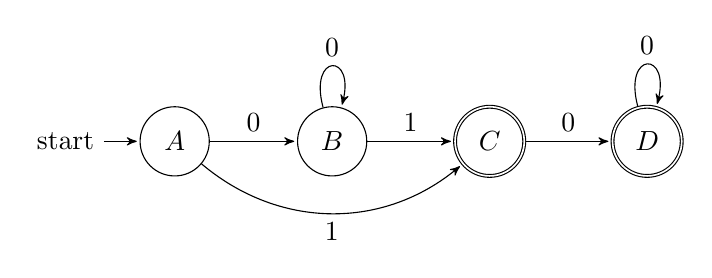
\begin{tikzpicture}[->,>=stealth',shorten >=1pt,auto,node distance=2cm,
        scale = 1,transform shape]

    \node[state,initial] (A) {$A$};
    \node[state] (B) [right of=A]  {$B$};
    \node[state,accepting] (C) [right of=B]  {$C$};
    \node[state,accepting] (D) [right of=C] {$D$};

    \path (A) edge              node {$0$} (B);
    \path (A) edge[below,bend right=40]  node {$1$} (C);
    \path (B) edge[loop above]              node {$0$} (B);
    \path (B) edge            node {$1$} (C);
    \path (C) edge              node {$0$} (D);
    \path (D) edge[loop above]              node {$0$} (D);

    \end{tikzpicture}
    
    \noindent(3)\\
     \indent$\Pi_0=\{\{A,B\},\{C,D\}\}$  \\
    \indent 合并等价态$A\sim B$,$C\sim D$
    
    
     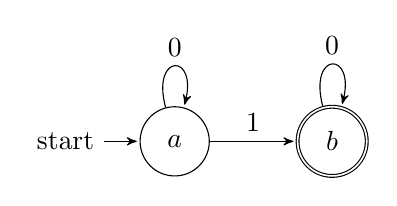
\begin{tikzpicture}[->,>=stealth',shorten >=1pt,auto,node distance=2cm,
        scale = 1,transform shape]

    \node[state,initial] (0) {$a$};
    \node[state,accepting] (1) [right of=0]  {$b$};

    \path (0) edge[loop above]              node {$0$} (0);
    \path (0) edge            node {$1$} (1);
    \path (1) edge[loop above]              node {$0$} (1);

    \end{tikzpicture}
    
    \noindent(4)\\
     \indent$R_{00}^{-1}=0|\epsilon$\\
    \indent$R_{01}^{-1}=1$\\
    \indent$R_{10}^{-1}=\varnothing$\\
    \indent$R_{11}^{-1}=0|\epsilon$\\
    
    \indent step 0\\
    \indent$R_{00}^{0}=R_{00}^{-1}(R_{00}^{-1})^*R_{00}^{-1}|R_{00}^{-1}=(0|\epsilon)(0|\epsilon)^*(0|\epsilon)|(0|\epsilon)=0^*$\\
    \indent$R_{01}^{0}=R_{00}^{-1}(R_{00}^{-1})^*R_{01}^{-1}|R_{01}^{-1}=(0|\epsilon)(0|\epsilon)^*1|1=0^*1$\\
    \indent$R_{10}^{0}=R_{10}^{-1}(R_{00}^{-1})^*R_{00}^{-1}|R_{10}^{-1}=\varnothing(0|\epsilon)^*(0|\epsilon)|\varnothing=\varnothing$\\
    \indent$R_{11}^{0}=R_{10}^{-1}(R_{00}^{-1})^*R_{01}^{-1}|R_{11}^{-1}=\varnothing(0|\epsilon)^*1|(0|\epsilon)=0|\epsilon$\\
    
    \indent step 1\\
    \indent$R_{00}^{1}=R_{01}^{0}(R_{11}^{0})^*R_{10}^{0}|R_{00}^{0}=0^*1(0|\epsilon)^*\varnothing|0^*=0^*$\\
    \indent$R_{01}^{1}=R_{01}^{0}(R_{11}^{0})^*R_{11}^{0}|R_{01}^{0}=0^*1(0|\epsilon)^*(0|\epsilon)|0^*1=0^*10^*$\\
    \indent$R_{10}^{1}=R_{11}^{0}(R_{11}^{0})^*R_{10}^{0}|R_{10}^{0}=(0|\epsilon)(0|\epsilon)^*\varnothing|\varnothing=\varnothing$\\
    \indent$R_{11}^{1}=R_{11}^{0}(R_{11}^{0})^*R_{11}^{0}|R_{11}^{0}=(0|\epsilon)(0|\epsilon)^*(0|\epsilon)|(0|\epsilon)=0^*$\\\\
    \indent 所以\\
    \indent$r^{'}=|_{s_j\in{F_D}}R_{0j}^{|S_D|-1}=R_{01}^{1}=0^*10^*$\\
    
    \noindent(5)\\
    相同
    
    
\end{solution}
%%%%%%%%%%%%%%%

%%%%%%%%%%%%%%%%%%%%
% 如果没有需要订正的题目,可以把这部分删掉

% \begincorrection
%%%%%%%%%%%%%%%%%%%%

%%%%%%%%%%%%%%%%%%%%
% 如果没有反馈,可以把这部分删掉
\beginfb

你可以写 (若无内容, 可删除该节)
\begin{itemize}
  \item 对课程及教师的建议与意见
  \item 教材中不理解的内容
  \item 希望深入了解的内容
  \item $\cdots$
\end{itemize}
%%%%%%%%%%%%%%%%%%%%
\end{document}